\documentclass[12pt]{article}
\usepackage[english]{babel}
\usepackage[utf8x]{inputenc}
\usepackage{amsmath}
\usepackage{graphicx}
\usepackage[colorinlistoftodos]{todonotes}
\usepackage[font=small,labelfont=bf]{caption}
\graphicspath{ {images/} }

\begin{document}

\begin{titlepage}

\newcommand{\HRule}{\rule{\linewidth}{0.5mm}} % Defines a new command for the horizontal lines, change thickness here

\center % Center everything on the page
 
%----------------------------------------------------------------------------------------
%	HEADING SECTIONS
%----------------------------------------------------------------------------------------

\textsc{\LARGE Edinburgh Napier University}\\[1.5cm] % Name of your university/college
\textsc{\large SET09121}\\[0.5cm] % Minor heading such as course title

%----------------------------------------------------------------------------------------
%	TITLE SECTION
%----------------------------------------------------------------------------------------

\HRule \\[0.4cm]
{ \huge \bfseries Games Engineering - Final Report}\\[0.4cm] % Title of your document
\HRule \\[1.5cm]
 
%----------------------------------------------------------------------------------------
%	AUTHOR SECTION
%----------------------------------------------------------------------------------------

\vfill % Fill the rest of the page with whitespace
\textsc{Developers:}\\[0.5cm]
Stephan Aldhous - 40288816
\linebreak
Glenn Wilkie-Sullivan - 40208762
\linebreak

\end{titlepage}

\section{Introduction}

Rogue: 2125 is a rogue-like top down shooter game which incorporates tile mapping, resource management and statistical awareness such as skills and levels. The game sees the player dungeon crawling through innumerable procedurally generated levels which scale in difficulty as the game progresses. The player will have to kill enemies, discover secrets, enhance abilities and find the secret artifacts of the game to level up. These secrets will be in the form of hidden rooms which house better rewards for the player, like equipment or powerups. With this comes a high risk though - these rooms will naturally be more dangerous, if the player is feeling adventurous. \linebreak

Our scope was somewhat ambitious, but trying to keep the complex features realistic, robust and easy to understand. Within this specific genre of game, there is a very wide range of possibilities for features and gameplay components, which means the game could be infinitely big, or lightweight and small. Rogue: 2125 is a nice blend of both - the overarching gameplay is lightweight, easy to understand and fulfilling in reward - however, the backend features, namely tile generation, is complex in design and implementation. \linebreak

In terms of inspiration, the game draws certain gameplay points from games such as Rogue Fable II (kongregate.com) and Hotline Miami by Dennaton Games. Mainly, Rogue Fable II offers a range of well designed RPG elements which seemed applicable to apply in our game. The resource management within RF2 sees the player tracking health, energy and hunger - this adds a unique difficulty mechanic, which we were interested in implementing for our game through health, fuel and experience. Another interesting gameplay mechanic we implemented was status effects from tiles - heavily influenced from RF2, which has a similar feature. Some tiles can slow, damage, poison, etc. which is another avenue to add replayability and authenticity. The game unfortunately never got to see fully working tiles, but in the future, the game may have them implemented. As stated before, Rogue: 2125 also draws inspiration from Hotline Miami; the game has a very unique pace to it which sets a very frantic style of movement, hopefully achievable with our game in combination with the unique status effects of the tiles and enemies.

\clearpage

\section{Game Design Document Changes and Omissions}

Within our game design document, we followed a slightly altered form of the MoSCoW prioritisation structure. Instead of prioritising by importance, we structed it by what we invisioned the easiest to hardest features to look like. However, some of the features that were promised were not delivered. To start with, only very basic enemies were implemented, without AI or any kind of prevention functions. This leads to the next promised feature - pickups from enemies. When killed, enemies were meant to drop a variance of items to help the player; while we had the work in place to implement this, it needed a bit more work to be fully functional, and is unfortunately absent from the game. The game unfortunately doesn't have any form of experience points either - therefore, there is no way to level up and no way for the player to progress. Again, while work was in place to implement player stats/equipment/etc, unfortunately the game has no statistical balance/difficulty spiking. \newline

The game has no items or resources, therefore a UI was naturally not implemented, except for the menus. The game has no visible exits/separate rooms or end condition, although one could be easily implemented given extra time.

\clearpage

\section{Software Design}

The game at it's core is very simple, given that it has no win/end condition. Starting with the menus, it was planned to have four menus - main, settings, highscores and pause. The main menu and settings menus are (almost) fully functional - with transitions implemented. \newline

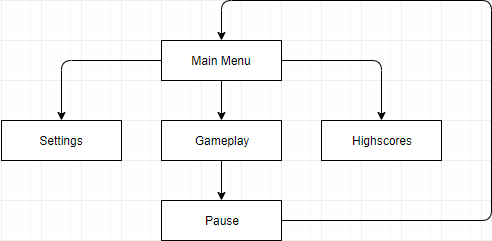
\includegraphics[width=\textwidth,height=\textheight,keepaspectratio]{MenuState}
\captionof{figure}{Menu States}

\hspace{1cm}

Unfortunately, highscores as well as pausing aren't quite implemented in the game, although the functionality for saving a game is almost there. While playing the game, unfortunately only a few states are available, not warranting a separate diagram - idle, move and shoot. With more functionality, the tank in the game could boost/explode/power-up/etc.

\clearpage

\section{Game Implementation}



\end{document}